% !TeX root = ./corona_contact_tracing.tex
% chktex-file 46
% !TeX spellcheck = en-GB
% !TeX encoding = utf8

\subsection{SIR Model}
Our basic stochastic SIR model relies on the assumptions that every person in an environment can be modeled as a point value, which has a location (i.e.\ GPS coordinates) and an infection state. These states can be either \textit{susceptible} (S), \textit{infected} (I), \textit{recovered} (R) or in advanced models also \textit{under quarantine} (Q) or \textit{dead} (D). All individuals, here called agents, have a probability (here called diffusion rate $d$ to make a step per time step on a predefined grid. In the case, that some agents meet at the same location, disease spreading can occur. An infected agent spreads the disease with probability $\beta$ to all the agents in its close vicinity (same location on the grid). Furthermore recovery is covered by taking a recovery rate into account, i.e.\ a probability $\gamma$ to recover from the disease per time step. If an infected agent recovers from the disease, the state of the agent changes from \textit{infected} to \textit{recovered}, which is definite (no double infections). The process ends, when no infected agents are left.
\begin{center}
    Susceptibles $\overset{\beta}{\longrightarrow}$ Infected $\overset{\gamma}{\longrightarrow}$ Recovered.
\end{center}

An example of a early model state is shown in Figure~\ref{fig:1}
\begin{figure}[H]
    \centering
    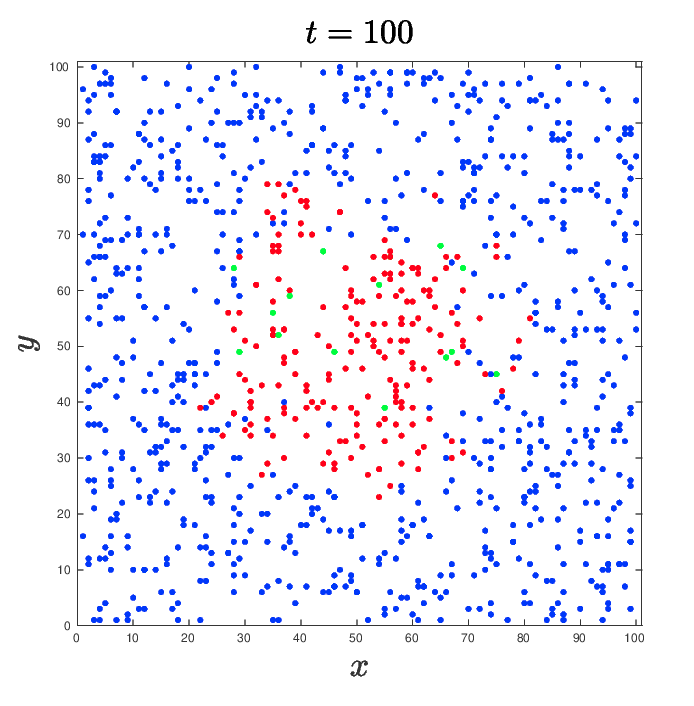
\includegraphics[width=0.4\linewidth]{initial_setup.png}
    \caption{Early state of SIR model, blue dots = susceptibles, red dots = infected agents, green dots = Recovered agents}%
    \label{fig:1}
\end{figure}

In this case, 1000 agents were initialized on a 100 by 100 grid, where a certain amount of infected agents were introduced as a seed. Letting the agents perform random walks on the grid (maximally one step each time step with probability $d$), and letting the model converge, the results in figure~\ref{fig:2} can be observed.

\begin{figure}[H]
    \centering
    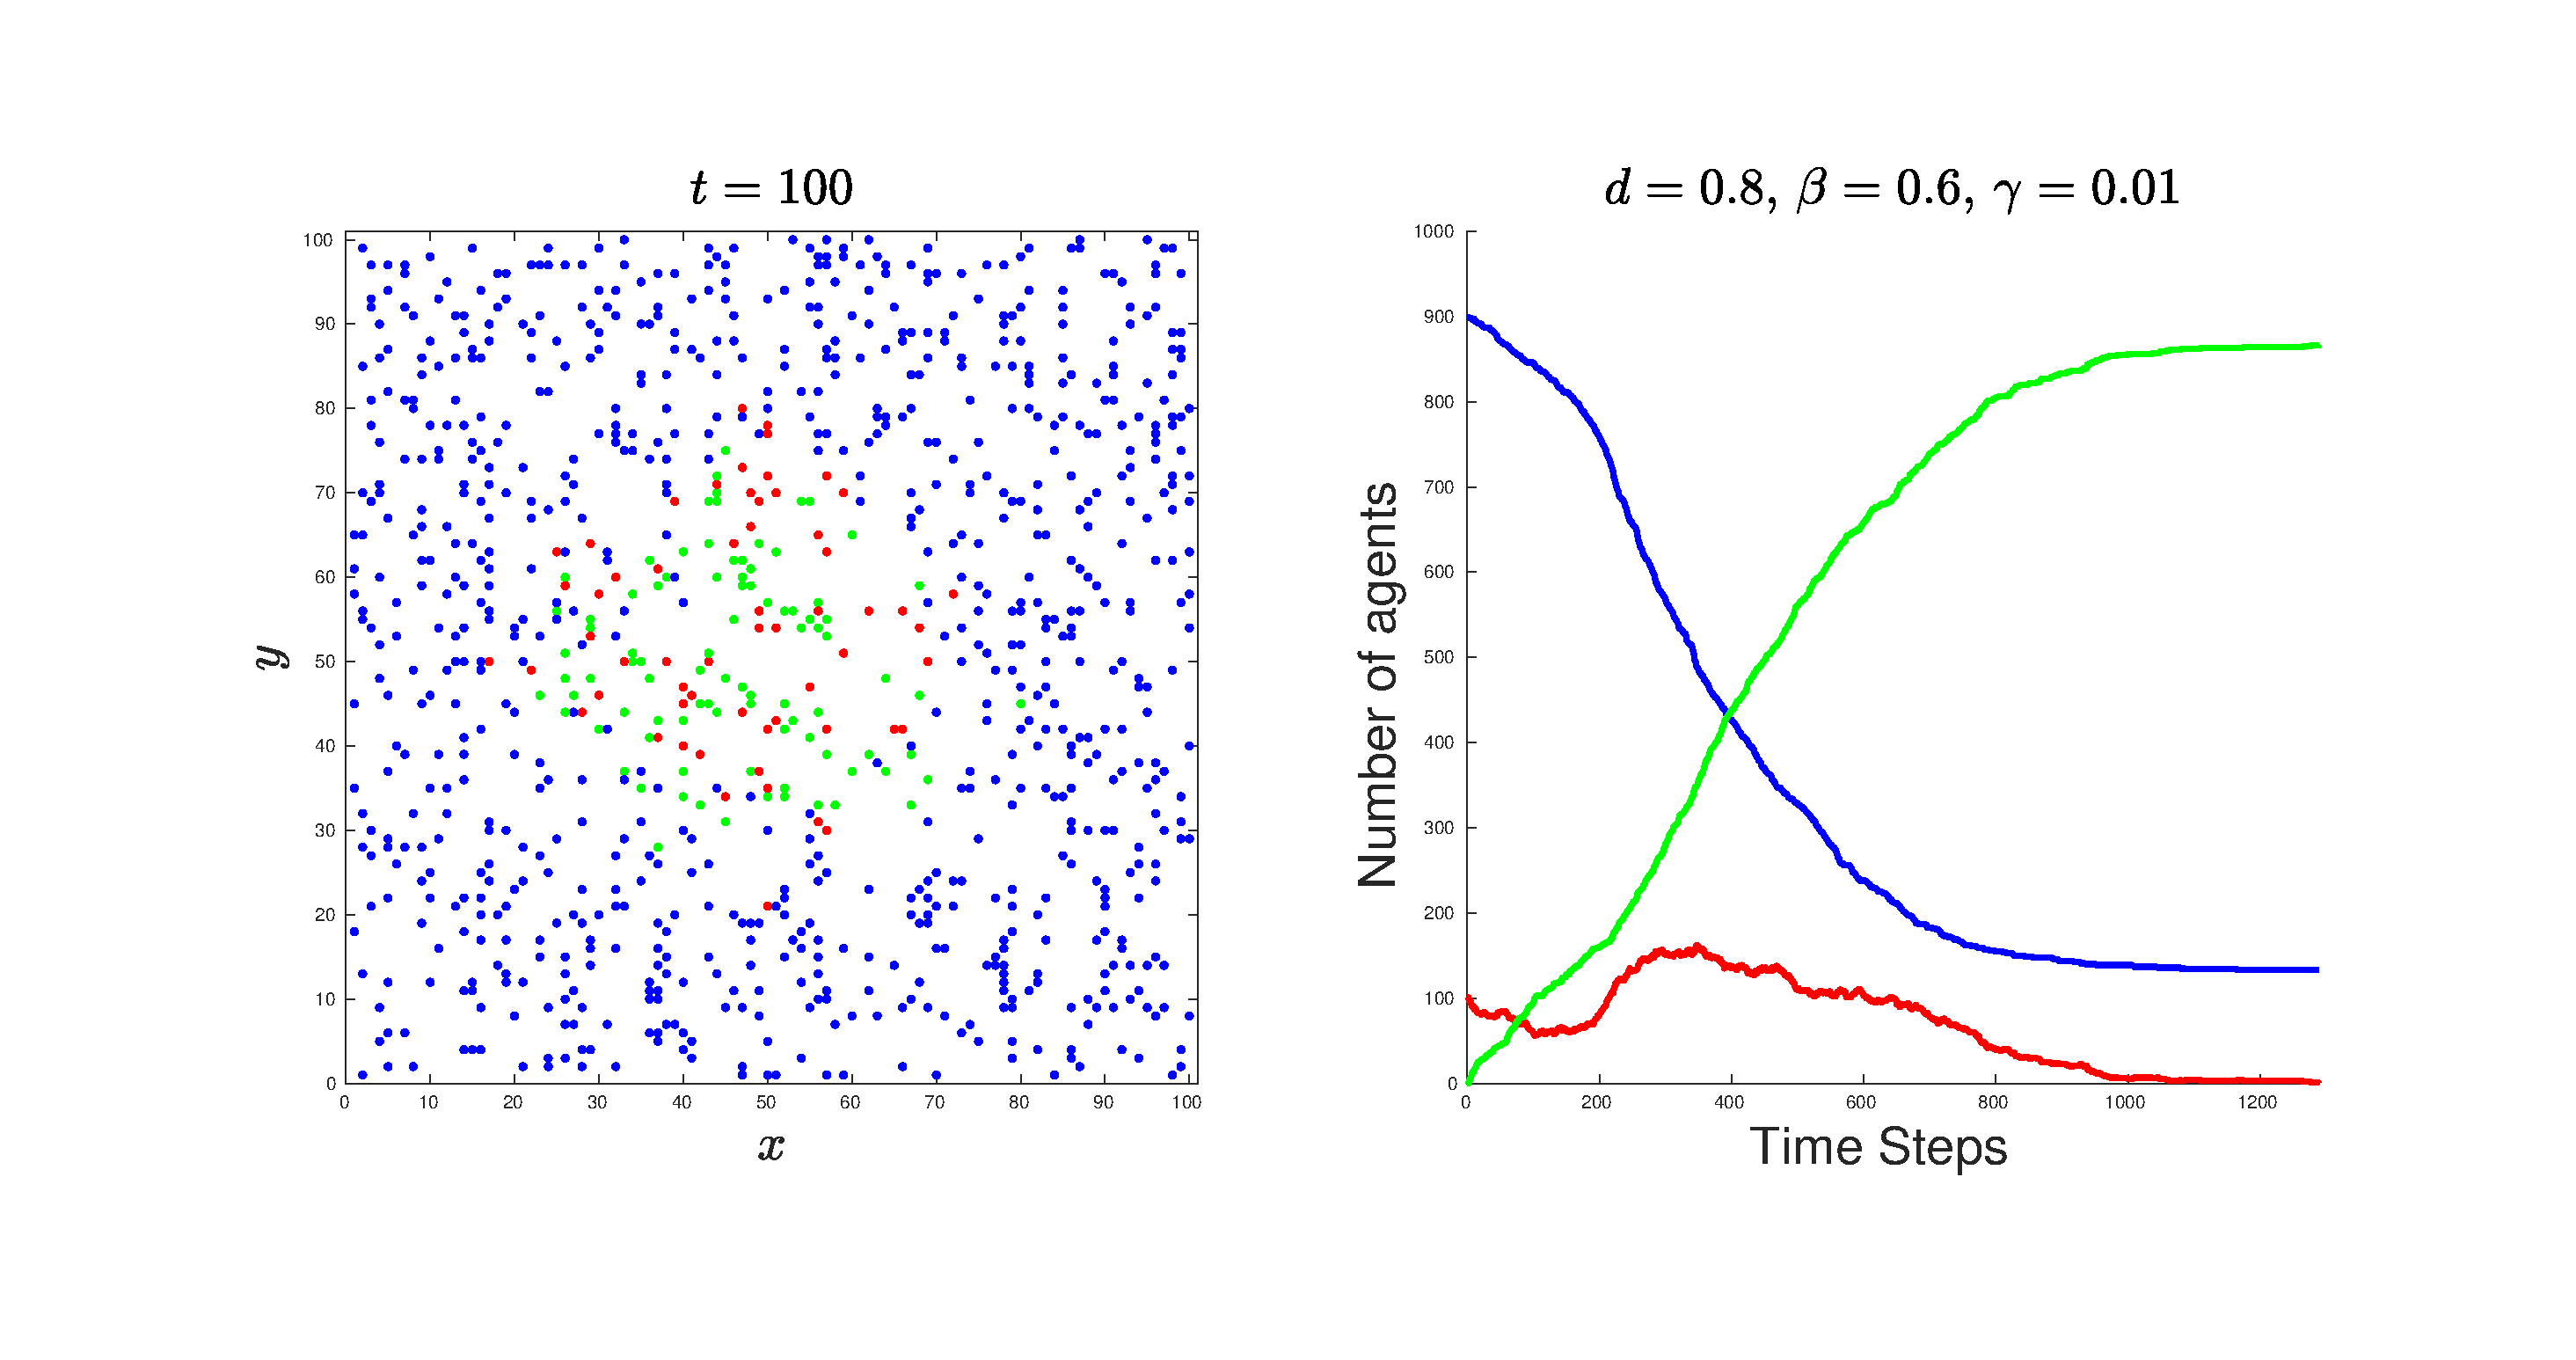
\includegraphics[width=0.9\linewidth]{1_1000_agents}
    \caption{Plot of the proportions of susceptible (blue), infected (red) and recovered (green) individuals in each state over time.}%
    \label{fig:2}
\end{figure}

With the above stated parameters ($d=0.8$, $\beta=0.6$, $\gamma=0.01$), the disease does not spread over the whole population. However over 80\% were infected over time, which could be a very likely scenario of the corona out brake.